\chapter{Optimization of steam generating system}
\section{Steam generator subsystem}

In a solar parabolic trough power plant in which intermediate heat-transfer fluid (take oil for instance) is used, heat addition to the working fluid (take water for instance) takes place in three counterflow heat exchangers (steam generator subsystem, SGSS) as shown in Figure~\ref{fig:PTC}. The SGSS is consist of preheater, evaporator, superheater. The flow rates of both oil and water remains the same in the three heat exchangers. 
The water has phase change in the three heat exchangers, from liquid to vapor in the evaporator, however, oil remains liquid. The heat capacity of water in each heat exchanger differs a lot. The heat capacity of oil has no significant difference since no phase change. The heat transfer process is illustrated on Figure~\ref{fig:DeltaTmin}. Large temperature differences exist at the inlets and outlets of the heat exchangers, which makes large entropy production during the entire heat exchange process.


\noindent \begin{figure}[htbp]
\begin{center}
	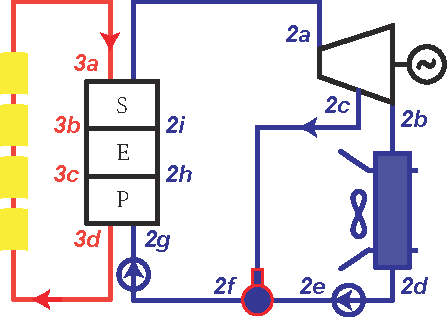
\includegraphics[width = 0.7\columnwidth]{fig/PTC}
	\caption{An typical solar parabolic trough system}
	\label{fig:PTC}
\end{center}
\end{figure}

\noindent \begin{figure}[htbp]
\begin{center}
	\includegraphics[width = 0.7\columnwidth]{fig/DeltaTmin}
	\caption{The steam generating process in countertlow heat exchangers}
	\label{fig:DeltaTmin}
\end{center}
\end{figure}

The heat-transfer fluid at $3a$ represents the solar field outlet temperature and at $3d$, the field return temperature. The difference between these can be reduced by increasing the flow rate of heat-transfer fluid through the field and thus the parasitic pumping power.

Since the heat exchangers must always stay a positive temperature difference for heat transfer, the temperature of oil must always be higher than the temperature of water. On the other hand, the temperature of oil should not be much higher that that of the water. Higher oil temperature leads more heat losses in the solar field hence lower efficiency, more entropy production generated in the heat exchange process. Besides, higher oil temperature brings greater operational risks for the solar system. Setting the appropriate temperature difference between the oil and water is particularly important. The oil temperature must always higher (but no too much higher) than that of the water.

To find out the inlet and outlet temperatures of oil at the solar field, the lowest temperature difference of oil and water is defined as the pinch temperature $\Delta T_{min}$. The temperatures of state points $2h$ and $2i$ are determined by the main pressure of the steam turbine in Figure~\ref{fig:PTC}, and $T_{3b}$ is larger than $T_{3c}$. So state points $3c$ and $2h$, called the pinch point, are set to satisfy the pinch temperature, $T_{3c} - T_{2h} = \Delta T_{min}$. The pinch temperature $\Delta T_{min}$ is usually set to be 10$\sim$20$\,\mathrm{K}$.
It has to be mentioned that the temperature differences $T_{3d} - T_{2g}$ and $T_{3a} - T_{2j}$ worth attention to be not larger than $\Delta T_{min}$.

However, even with the chosen pinch temperature $\Delta T_{min}$, the temperature difference during the heat exchange process in SGSS is still large due to the phase change of water. Large temperature differences always exists at the inlet/outlet of the exchangers. As shown in Figure~\ref{fig:DeltaT}, it is a tradeoff to choose a mass flow rate of oil ($\dot{m}_3$). $\dot{m}_3$ affects the slope of curve $3a$-$3b$-$3c$-$3d$. A smaller $\dot{m}_3$ leads to a steeper curve, hence a larger $T_{3a} - T_{2j}$. A larger $\dot{m}_3$ leads to a more gentle curve, hence a larger $T_{3d} - T_{2g}$. The heat transfer processes in SGSS always produce large entropy and exergy losses. In this regard, a new steam generating system to reduce exergy loss is put forward.

\noindent \begin{figure}[htbp]
\begin{center}
	\includegraphics[width = 0.7\columnwidth]{fig/DeltaT}
	\caption{The tradeoff to choose $\dot{m}_3$}
	\label{fig:DeltaT}
\end{center}
\end{figure}

\section{Multi-stage exergy loss reduction system}\label{sec:mers}
The reason of large temperature differences of the two curves in Figure~\ref{fig:DeltaTmin} is that, the slope of oil curve changes slightly in different heat exchangers (preheater, evaporator and superheater), while the water curve changes dramatically due to large heat capacity $c_p$ differences.

\begin{equation}
  \Delta Q =  c_p\dot{m} \Delta T
\end{equation}

The slope of the curves are determined by $c_p\dot{m}$, $\dot{m}$ can be altered to adjust the slope of the curves despite the $c_p$ is unalterable. All the water needs to be heated from supercooled water to superheated steam, which means $\dot{m}_2$ remains the same in the three heat exchangers. The last way is to change $\dot{m}_3$ in the heat exchangers.

\noindent \begin{figure}[htbp]
\begin{center}
	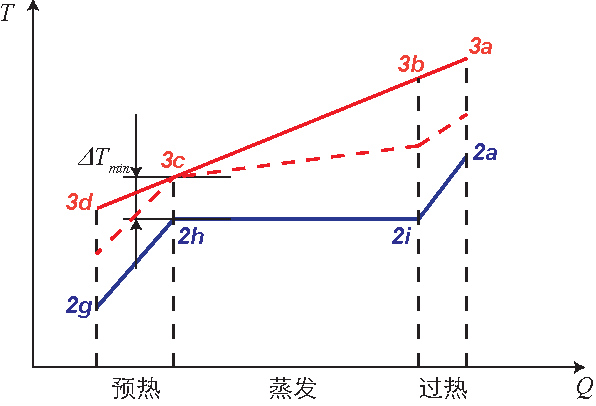
\includegraphics[width = 0.7\columnwidth]{fig/BetterCurve}
	\caption{Change $\dot{m}_3$ in the heat exchangers to reduce the temperature difference}
	\label{fig:BetterCurve}
\end{center}
\end{figure}

As shown in Figure~\ref{fig:BetterCurve}, the oil curve can be changed to the dashed curve. The temperature difference between the water curve and oil curve reduces significantly. Water is heated in three stages and the exergy loss reduces. The corresponding steam generating system is so called Multi-stage exergy loss reduction system (MERS).
Figure~\ref{fig:SEP} shows the schematic diagram of the MERS for comparison of typical solar parabolic trough system in Figure~\ref{fig:PTC}. The solar field in Figure~\ref{fig:PTC} has been divided into three independent sectors. Each sector becomes the heat source of a range for the steam heating process: the first corresponds to overheating, the second to evaporation, and the third to preheating. 
%Each section can be equipped with a thermal storage system to overcome the instability and intermittency of solar energy.
It has to be mentioned that the collectors in the schematic diagram are only used for explanation. The arrangement of these collectors can be in series, in parallel or combination of both.

\noindent \begin{figure}[htbp]
\begin{center}
	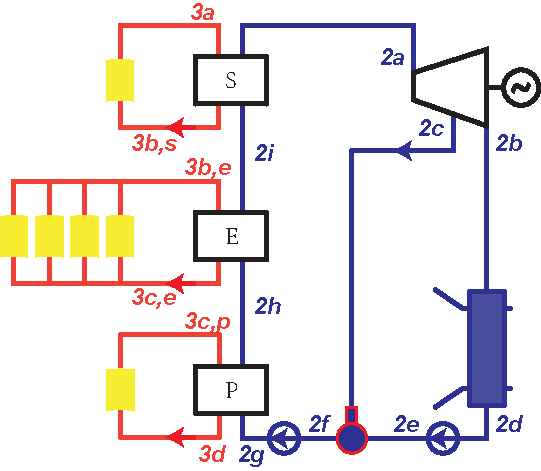
\includegraphics[width = 0.7\columnwidth]{fig/SEP}
	\caption{The schematic diagram of the MERS}
	\label{fig:SEP}
\end{center}
\end{figure}

To optimize the MERS, considering the limitation of pinch temperature, temperatures of the oil at the inlet/outlet of the heat exchangers can be set according to following rules:
\begin{eqnarray*}
	&T_{3d} - T_{2g} = \Delta T_{min}\\
   &T_{3c,p} = T_{3c,e} = T_{3c}\\
   &T_{3c} - T_{2h} = \Delta T_{min}\\
	&T_{3b,e} = T_{3b,s} = T_{3b}\\
	&T_{3a} - T_{2a} = \Delta T_{min}
\end{eqnarray*}


A large flow rate of oil in the evaporator $\dot{m}_{3,e}$ can be applied to decrease the temperature $T_{3b}$ hence the temperature differences of the oil and water. However, a large $\dot{m}_{3,e}$ requires more oil usage and more pump power for the oil circuits. Besides, $\dot{m}_{3,e}$ is limited for the limitation of oil velocity in the pipes.

The enthalpy of each state point can be determined by its temperature and pressure.

The optimum oil average temperature in the solar field corresponds to the preheater is
\begin{equation}
  T_{3,p} = (T_{2g} + T_{2h})/2 + \Delta T_{min}
\end{equation}

The optimum oil flow rate in the solar field corresponds to the preheater is
\begin{equation}
  \dot{m}_{3,p} = \dot{m}_{2}(h_{2h} - h_{2g})/(h_{3c} - h_{3d})
\end{equation}

The optimum oil average temperature in the solar field corresponds to the evaporator is
\begin{equation}
  T_{3,e} = (T_{3b} + T_{3c})/2
\end{equation}

The optimum oil flow rate in the solar field corresponds to the evaporator is
\begin{equation}\label{eq:m_3e}
  \dot{m}_{3,e} = \dot{m}_{2}(h_{2i} - h_{2h})/(h_{3b} - h_{3c})
\end{equation}

The optimum oil average temperature in the solar field corresponds to the superheater is
\begin{equation}
  T_{3,s} = (T_{3b} + T_{2a} + \Delta T_{min})/2
\end{equation}

The optimum oil flow rate in the solar field corresponds to the superheater is
\begin{equation}
  \dot{m}_{3,s} = \dot{m}_{2}(h_{2a} - h_{2i})/(h_{3a} - h_{3b})
\end{equation}

\section{Comparison}

To find out the effect of MERS, models of traditional SGSS and proposed MERS are developed based on the models of the components. To clear find out the influence of oil temperature on the performance of the trough collectors, the equation summarized by~\cite{Rovira2011} is used.
\begin{equation}
  \eta(T) =  0.69563 + 0.000313T - 0.0000013T^2
\end{equation}
where $T$ is the average temperature of the tube. Since the $Nu$ number in the tube is large (about 1$\times$10$^4$), small temperature difference exists between the absorber and oil. So the average oil temperature can be used as the average value of the tube.

The exergy loss caused by a heat exchange process per unit time
\begin{equation}
  \dot{I} = T_amb (\sum \dot{m}_os_o - \sum \dot{m}_is_i)
\end{equation}


The turbine and deaerator are the same for the two systems (SGSS and MERS), so that the corresponding state points of water are the same. The main parameters are listed in Table~\ref{tab:ptc}.
\begin{table}[htbp]
	\caption{Main parameters used for both SGSS and MERS}
	\begin{center}
	\begin{tabular}{cccc}
		\toprule
		Parameter		&	Value	&	Parameter		&	Value\\
		\midrule
		$I_r$	&	700$\,\mathrm{W/m^2}$	&	$T_s$		&	613.15$\,\mathrm{K}$\\
		$P_{ge}$	&	6$\times$10$^6\,\mathrm{W}$	&	$p_s$		&	2.35$\times$10$^6\,\mathrm{Pa}$\\
		$\eta_{i,tb}$	&	0.711	&	$p_c$		&	1.5$\times$10$^4\,\mathrm{Pa}$\\
		$\eta_{ge}$	&	0.975	&	$p_{de}$		&	1$\times$10$^6\,\mathrm{Pa}$\\
		$\Delta T_{min}$	&	15$\,\mathrm{K}$	&	&\\		
		\bottomrule
	\end{tabular}
	\end{center}
	\label{tab:ptc}
\end{table}
\noindent \begin{figure}[htbp]
\begin{center}
	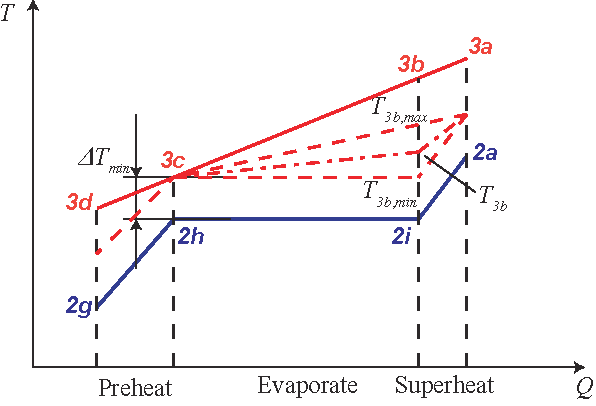
\includegraphics[width = 0.7\columnwidth]{fig/T3b}
	\caption{$T_{3b}$ in the $T$-$Q$ diagram of the heat transfer processes}
	\label{fig:T3b}
\end{center}
\end{figure}

As discussed in Section~\ref{sec:mers}, $T_{3b}$ is an undetermined value. Figure~\ref{fig:T3b} shows the minimum and maximum value of it. $T_{3b,min}$ means the limit situation of unlimited flow rate of oil in the evaporator, $T_{3b,min} = T_{3c}$. (see Equation~\ref{eq:m_3e}) $T_{max}$ has the traditional effect of temperature differences in the evaporator and superheater, $\dot{m}_{3,e} = \dot{m}_{3,s}$. In our research, $T_{3b}$ is set to be the average value of the two limitations, $T_{3b} = (T_{3b,min} + T_{3n,max}) / 2$.
\begin{equation}
  \dfrac{T_{b,max}-T_{3c}}{T_{3a} - T_{3c}} = \dfrac{T'_{3b} - T_{3c}}{T'_{3a} - T_{3c}}
\end{equation}

where $T'_{3a}$ and $T'_{3b}$ are the inlet oil temperature of superheater and evaporator in SGSS respectively.
\begin{table}[htbp]
	\caption{Simulation results of SGSS and MERS}
	\begin{center}
	\begin{tabular}{ccc}
		\toprule
		&    SGSS	&	MERS\\
		\midrule
		$T_{2a}$	&	613.15$\,\mathrm{K}$	&	613.15$\,\mathrm{K}$\\
		$T_{2i}$	&	493.83$\,\mathrm{K}$	&	493.83$\,\mathrm{K}$\\
		$T_{2h}$	&	493.83$\,\mathrm{K}$	&	493.83$\,\mathrm{K}$\\
		$T_{2g}$	&	453.28$\,\mathrm{K}$	&	453.28$\,\mathrm{K}$\\
		$T_{3a}$	&	653.15$\,\mathrm{K}$	&	628.15$\,\mathrm{K}$\\
		$T_{3b}$	&	634.11$\,\mathrm{K}$	&	560.62$\,\mathrm{K}$\\
		$T_{3c}$	&	508.83$\,\mathrm{K}$	&	508.83$\,\mathrm{K}$\\
		$T_{3d}$	&	495.43$\,\mathrm{K}$	&	468.28$\,\mathrm{K}$\\
		$\dot{m}_{3p}$	&	47.8$\,\mathrm{kg}$	&	16.1$\,\mathrm{kg}$\\
		$\dot{m}_{3e}$	&	47.8$\,\mathrm{kg}$	&	120.8$\,\mathrm{kg}$\\
		$\dot{m}_{3s}$	&	47.8$\,\mathrm{kg}$	&	14.3$\,\mathrm{kg}$\\
		$\dot{I}_p$    &    4.79$\times$10$^4\,\mathrm{W}$    &    2.39$\times$10$^4\,\mathrm{W}$\\
		$\dot{I}_e$    &    1.10$\times$10$^6\,\mathrm{W}$    &    6.26$\times$10$^5\,\mathrm{W}$\\
		$\dot{I}_s$    &    1.80$\times$10$^5\,\mathrm{W}$    &    9.19$\times$10$^4\,\mathrm{W}$\\
		$\dot{I}_{total}$    &    1.33$\times$10$^6\,\mathrm{W}$    &    7.42$\times$10$^5\,\mathrm{W}$\\
		$\eta_p$    &    0.525    &    0.538\\
		$\eta_e$    &    0.450    &    0.491\\
		$\eta_s$    &    0.359    &    0.422\\
		$\eta_{total}$    &    0.440    &    0.484\\
		\bottomrule
	\end{tabular}
	\end{center}
	\label{tab:comparison}
\end{table}
Simulation results of the two system models are listed in Table~\ref{tab:comparison}. It can be found that the MERS can effectively reduce exergy loss hence improve the system efficiency compared to traditional SGSS.

%In a traditional solar parabolic trough power plant, the potential of exergy loss reduction in the heating process of Rankine cycle is large. There exist large temperature differences between the heat transfer fluid (HTF) and water in the steam generator subsystem (SGSS). In order to reduce the temperature differences, a novel multi-stage exergy loss reduction system (MERS) with different HTF flows to lower the required HTF temperature is put forward. A flow control strategy of HTF depending on the analytical system model was derived. Energy and exergy efficiency of the MERS was analyzed and compared with the SGSS of traditional solar parabolic trough power plant. Result shows that the MERS can effectively decrease the exergy loss in the heating process, thus the performance of the plant can be improved.


